\documentclass[a4paper]{article}
\usepackage[svgnames]{xcolor}
\usepackage{amsmath,amsfonts,amssymb}
\usepackage{geometry}
\usepackage{fancyhdr}
\usepackage{graphicx}
\usepackage{titlesec}
\usepackage{caption}
\usepackage{subcaption}
\usepackage{tikz}
\usepackage{tcolorbox}
\usepackage{float} % For figure positioning
\usepackage{lipsum}
\usepackage{mdframed}
\usepackage{amsmath}
\usepackage{amsmath,amsfonts,amssymb}
\usepackage{graphicx}
\usepackage{enumitem}
\usepackage{titlesec}
\usepackage{fancyhdr}
\usepackage{hyperref}
% \usepackage{floatrow}
\usepackage{listings}
\usepackage{geometry}
\usepackage{fancyhdr}
\usepackage{empheq}
\usepackage[svgnames]{xcolor}
\usepackage{xpatch}
\usepackage{listings}

\lstdefinestyle{Matlab}{
    language=Matlab,                      % Use MATLAB language
    basicstyle=\ttfamily\footnotesize,    % Font size and style
    keywordstyle=\color{blue},            % Color for keywords
    stringstyle=\color{red},              % Color for strings
    commentstyle=\color{green!50!black},  % Color for comments
    numbers=left,                         % Line numbers on the left
    numberstyle=\tiny\color{gray},        % Style of line numbers
    stepnumber=1,                         % Line numbers step
    numbersep=5pt,                        % Distance from line numbers
    frame=single,                         % Frame around the code
    tabsize=4,                            % Set tab size
    breaklines=true,                      % Automatic line breaking
    captionpos=b                          % Position of the caption
}


\geometry{margin=0.5in}
\pagestyle{fancy}
\fancyhf{}

% Header and Footer
% \fancyhead[L]{\includegraphics[width=1.5cm]{logo.png}} % Add your logo
\fancyhead[C]{\textbf{\color{blue!70}CS663 Assignment-3}}
% \fancyhead[R]{\color{blue!70}Saksham Rathi}
\fancyfoot[C]{\thepage}

% Custom Section Color and Format
\titleformat{\section}
{\color{purple!80!black}\normalfont\Large\bfseries}
{\thesection}{1em}{}

% Beautiful Title with TikZ
\newcommand{\cooltitle}[1]{%
  \begin{tikzpicture}
    \node[fill=blue!20,rounded corners=10pt,inner sep=10pt] (box)
    {\Huge \bfseries \color{black} #1};
  \end{tikzpicture}
}

% Stylish Solution Environment with float option enabled
% Stylish Solution Environment with breakable option
% Stylish Solution Environment with mdframed
\newenvironment{solution}[2][]{%
    \begin{mdframed}[linecolor=green!60!black, linewidth=2pt, roundcorner=10pt, backgroundcolor=green!5!white, skipabove=12pt, skipbelow=12pt]%
        \textbf{\large #2} % Heading in bold and large font
        \par\noindent\rule{\textwidth}{0.4pt} % Horizontal line after heading
        \vspace{0.5em} % Small vertical space
}{%
    \end{mdframed}%
}





\title{\cooltitle{CS663 Assignment-3}}
\author{{\bf Saksham Rathi, Kavya Gupta, Shravan Srinivasa Raghavan} \\
\small Department of Computer Science, \\
Indian Institute of Technology Bombay \\}
\date{}

\begin{document}

\maketitle
\section*{Question 4}

\begin{solution}{Solution}
    We have a $201\times 201$ image, where:
\begin{itemize}
    \item All pixels are black (value 0).
    \item The central column (column index 101) has all pixels with a value of 255.
\end{itemize}

Let $f(x, y)$ be the pixel value at position $(x, y)$:
\begin{itemize}
    \item For $x = 100$, $f(x, y) = 255$ for all $y$. (Assuming that our image indices are from 0 to 200.)
    \item For all other $x$, $f(x, y) = 0$ for all $y$.
\end{itemize}

Given a 2D image $f(x, y)$, its 2D DFT is defined as:
\begin{equation}
    F(u, v) = \frac{1}{\sqrt{MN}}\sum_{x=0}^{M-1} \sum_{y=0}^{N-1} f(x, y) e^{-j2\pi\left(\frac{ux}{M} + \frac{vy}{N}\right)}
\end{equation}

We are asked to find the 2D DFT of the given image.

\begin{equation}
    F(u, v) = \frac{1}{\sqrt{201\times 201}}\sum_{x=0}^{200} \sum_{y=0}^{200} f(x, y) e^{-j2\pi\left(\frac{ux}{201} + \frac{vy}{201}\right)}
\end{equation}

\begin{equation}
    F(u, v) = \frac{1}{\sqrt{201\times 201}} \sum_{y=0}^{200} 255\times e^{-j2\pi\left(\frac{u\times 100}{201}\right)} e^{-j2\pi\left(\frac{vy}{201}\right)}
\end{equation}

\begin{equation}
    F(u, v) = \frac{255\times e^{-j2\pi\left(\frac{u\times 100}{201}\right)}}{\sqrt{201\times 201}} \sum_{y=0}^{200} e^{-j2\pi\left(\frac{vy}{201}\right)}
\end{equation}

For $v = 0$, the sum is 201. For all other $v$:
\begin{equation}
    F(u, v) = \frac{255\times e^{-j2\pi\left(\frac{u\times 100}{201}\right)}}{\sqrt{201\times 201}} \frac{1-e^{-j2\pi\left(\frac{201v}{201}\right)}}{1-e^{-j2\pi\left(\frac{v}{201}\right)}}
\end{equation}

\begin{equation}
    F(u, v) = \frac{255\times e^{-j2\pi\left(\frac{u\times 100}{201}\right)}}{\sqrt{201\times 201}} \frac{1-1}{1-e^{-j2\pi\left(\frac{v}{201}\right)}} = 0
\end{equation}

So, the 2D DFT of the given image is:
\begin{equation}
    F(u, v) = \frac{255\times e^{-j2\pi\left(\frac{u\times 100}{201}\right)}}{\sqrt{201\times 201}} \times 201 \times \delta(v)
\end{equation}
where $\delta(v)$ is the Kronecker delta function (discrete image).
% \clearpage
\begin{lstlisting}[style=Matlab,caption={MATLAB code for Fourier Transform}]    
    F = fft2(image);
    F_shifted = fftshift(F);
    magnitude = abs(F_shifted);
    log_magnitude = log(1 + magnitude); % Logarithm for better visibility
    figure;
    imagesc(log_magnitude);
    title('Log Magnitude of Fourier Transform');
    xlabel('Frequency u');
    ylabel('Frequency v');
\end{lstlisting}

\clearpage
The MATLAB code for computing the 2D DFT of the given image is shown above.


\begin{figure}[H]
    \centering
    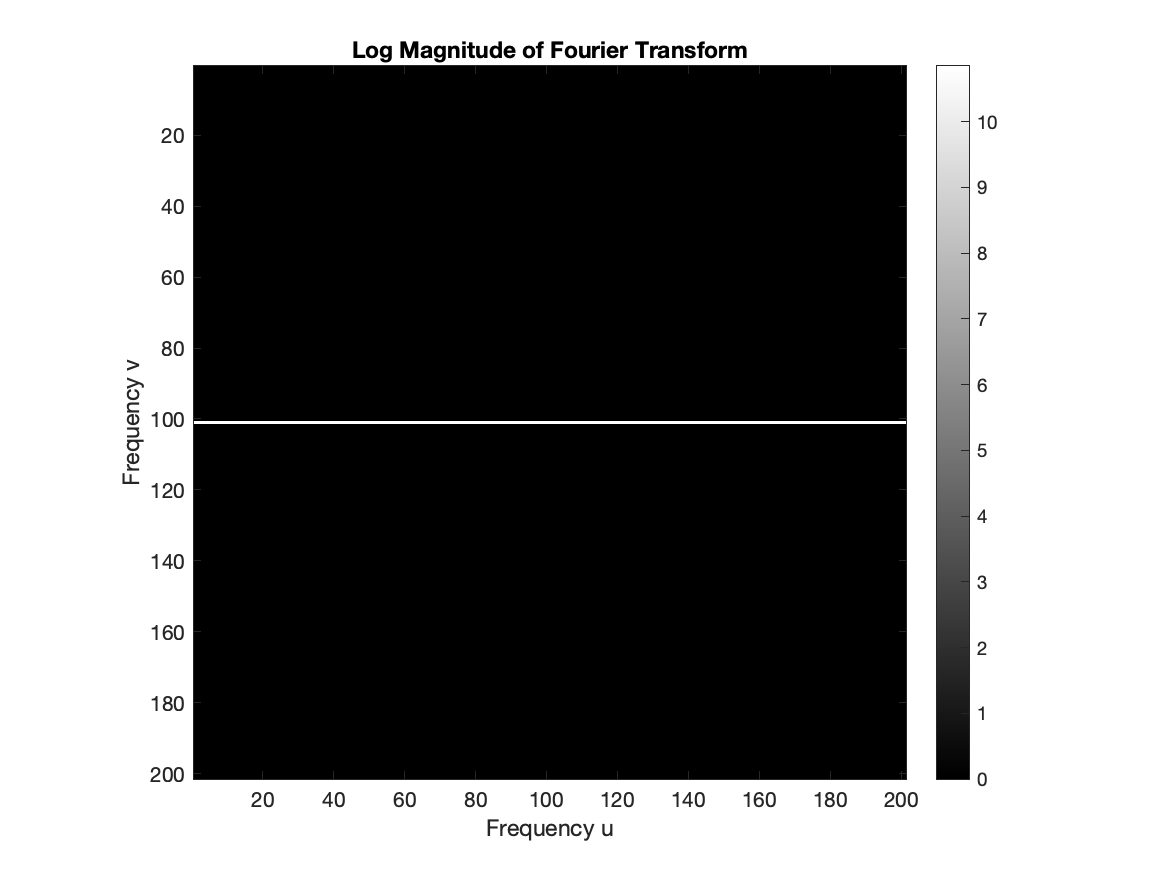
\includegraphics[width=0.8\textwidth]{../images/fourier_log_magnitude_image.png}
    \caption{Log Magnitude of Fourier Transform}
    \label{fig:fft}
\end{figure}


The vertical line is at $u = 100$ because of the fftshift we are doing. (If we comment out that line, the peak occurs at $u = 0$, which is what we have got from the mathematical derivation.)

\end{solution}


\end{document}
